% Important: If latex complains about unicode characters,
% please use "\usepackage[utf8x]{inputenc}" in your preamble
% You can change the size of the picture by putting it into the construct:
% 1) \resizebox{10cm}{!}{"below picture"} to scale horizontally to 10 cm
% 2) \resizebox{!}{15cm}{"below picture"} to scale vertically to 15 cm
% 3) \resizebox{10cm}{15cm}{"below picture"} a combination of above two
% It is not recomended to use the scale option of the tikzpicture environment.
\resizebox{!}{1.7cm}{
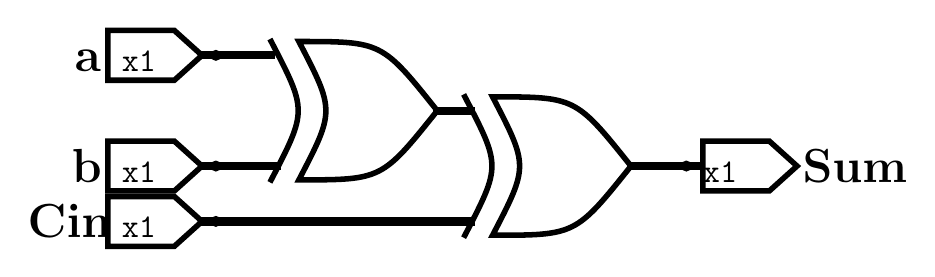
\begin{tikzpicture}[x=1pt,y=-1pt,line cap=rect]
\def\logisimfontA#1{\fontfamily{cmr}{#1}} % Replaced by logisim, original font was "SansSerif"
\def\logisimfontB#1{\fontfamily{cmtt}{#1}} % Replaced by logisim, original font was "Monospaced"
\definecolor{custcol_0_0_0}{RGB}{0, 0, 0}
\definecolor{custcol_ff_ff_ff}{RGB}{255, 255, 255}
\draw [line width=3.0pt, custcol_0_0_0 ]  (223.0,55.0) -- (243.0,55.0) ;
\draw [line width=2.0pt, custcol_0_0_0 ]  (153.0,35.0) .. controls  (133.0,10.0)  ..  (103.0,10.0) .. controls  (116.0,35.0)  ..  (103.0,60.0) .. controls  (133.0,60.0)  ..  (153.0,35.0) -- cycle ;
\draw [line width=2.0pt, custcol_0_0_0 ]  (93.0,10.0) .. controls  (106.0,35.0)  ..  (93.0,60.0) ;
\draw [line width=3.0pt, custcol_0_0_0 ]  (68.0,55.0) -- (73.0,55.0) -- (93.0,55.0) -- (95.0,55.0) ;
\draw [line width=2.0pt, custcol_0_0_0 ]  (58.0,64.0) -- (68.0,55.0) -- (58.0,46.0) -- (34.0,46.0) -- (34.0,64.0) -- cycle;
\logisimfontB{\fontsize{12pt}{12pt}\selectfont\node[inner sep=0, outer sep=0, custcol_0_0_0, anchor=base west] at  (39.0,61.0)  {x1};}
\logisimfontA{\fontsize{16pt}{16pt}\fontseries{bx}\selectfont\node[inner sep=0, outer sep=0, custcol_0_0_0, anchor=base west] at  (21.0,61.0)  {b};}
\fill [line width=2.0pt, custcol_0_0_0]  (73.0,55.0) ellipse (2.0 and 2.0 );
\draw [line width=3.0pt, custcol_0_0_0 ]  (68.0,15.0) -- (73.0,15.0) -- (93.0,15.0) -- (93.0,15.0) ;
\draw [line width=2.0pt, custcol_0_0_0 ]  (58.0,24.0) -- (68.0,15.0) -- (58.0,6.0) -- (34.0,6.0) -- (34.0,24.0) -- cycle;
\logisimfontB{\fontsize{12pt}{12pt}\selectfont\node[inner sep=0, outer sep=0, custcol_0_0_0, anchor=base west] at  (39.0,21.0)  {x1};}
\logisimfontA{\fontsize{16pt}{16pt}\fontseries{bx}\selectfont\node[inner sep=0, outer sep=0, custcol_0_0_0, anchor=base west] at  (22.0,21.0)  {a};}
\fill [line width=2.0pt, custcol_0_0_0]  (73.0,15.0) ellipse (2.0 and 2.0 );
\draw [line width=2.0pt, custcol_0_0_0 ]  (58.0,84.0) -- (68.0,75.0) -- (58.0,66.0) -- (34.0,66.0) -- (34.0,84.0) -- cycle;
\logisimfontB{\fontsize{12pt}{12pt}\selectfont\node[inner sep=0, outer sep=0, custcol_0_0_0, anchor=base west] at  (39.0,81.0)  {x1};}
\logisimfontA{\fontsize{16pt}{16pt}\fontseries{bx}\selectfont\node[inner sep=0, outer sep=0, custcol_0_0_0, anchor=base west] at  (5.0,81.0)  {Cin};}
\fill [line width=2.0pt, custcol_0_0_0]  (73.0,75.0) ellipse (2.0 and 2.0 );
\draw [line width=3.0pt, custcol_0_0_0 ]  (153.0,35.0) -- (163.0,35.0) -- (165.0,35.0) ;
\draw [line width=3.0pt, custcol_0_0_0 ]  (68.0,75.0) -- (73.0,75.0) -- (163.0,75.0) -- (165.0,75.0) ;
\draw [line width=2.0pt, custcol_0_0_0 ]  (223.0,55.0) .. controls  (203.0,30.0)  ..  (173.0,30.0) .. controls  (186.0,55.0)  ..  (173.0,80.0) .. controls  (203.0,80.0)  ..  (223.0,55.0) -- cycle ;
\draw [line width=2.0pt, custcol_0_0_0 ]  (163.0,30.0) .. controls  (176.0,55.0)  ..  (163.0,80.0) ;
\draw [line width=3.0pt, custcol_0_0_0 ]  (247.0,55.0) -- (244.0,55.0) ;
\draw [line width=2.0pt, custcol_0_0_0 ]  (273.0,46.0) -- (283.0,55.0) -- (273.0,64.0) -- (249.0,64.0) -- (249.0,46.0) -- cycle;
\logisimfontB{\fontsize{12pt}{12pt}\selectfont\node[inner sep=0, outer sep=0, custcol_0_0_0, anchor=base west] at  (249.0,61.0)  {x1};}
\logisimfontA{\fontsize{16pt}{16pt}\fontseries{bx}\selectfont\node[inner sep=0, outer sep=0, custcol_0_0_0, anchor=base west] at  (285.0,61.0)  {Sum};}
\fill [line width=2.0pt, custcol_0_0_0]  (243.0,55.0) ellipse (2.0 and 2.0 );
\end{tikzpicture}
}
